% Created 2024-08-29 Thu 15:38
% Intended LaTeX compiler: pdflatex
\documentclass[12pt]{article}
\usepackage[utf8]{inputenc}
\usepackage[T1]{fontenc}
\usepackage{graphicx}
\usepackage{longtable}
\usepackage{wrapfig}
\usepackage{rotating}
\usepackage[normalem]{ulem}
\usepackage{amsmath}
\usepackage{amssymb}
\usepackage{capt-of}
\usepackage{hyperref}
\usepackage[margin=1in]{geometry} \usepackage{amsmath}
\author{Jason Press}
\date{\today}
\title{Dropping Balls Onto the Floor}
\hypersetup{
 pdfauthor={Jason Press},
 pdftitle={Dropping Balls Onto the Floor},
 pdfkeywords={},
 pdfsubject={},
 pdfcreator={Emacs 29.4 (Org mode 9.8)}, 
 pdflang={English}}
\begin{document}

\maketitle
\begin{abstract}

\end{abstract}
\section{Introduction}
\label{sec:orgc815741}

The aim of this lab is to measure the acceleration of an object in free fall due to the gravitational force of Earth. In order to measure the acceleration due to gravity, two tests were performed: dropping a metal ball from a Drop Box and timing and measuring the distance it fell; and dropping a tennis ball from a balcony and timing the distance it fell.

Kinematics can describe the distance an object travels with constant acceleration as a function of time with \(x\left(t\right) = x_{0} + v_{0}t + \frac{1}{2}at^{2}\), where \(x_{0}\) is the initial position, \(v_{0}\) is the initial velocity, and \(a\) is the acceleration of the object. Assuming \(x_{0}\) is the initial height of the bottom of the ball \(h\), the end position of the ball is zero, \(v_{0}\) is zero since the ball starts at rest, and \(a\) is the negative acceleration of the ball due to gravity since objects fall down, then the kinematics equation can be rearranged to describe the acceleration due to gravity:

\begin{enumerate}
\item \(x(t) = x_{0} + v_{0}t + \frac{1}{2}at^{2} \)
\item \( \text{Assume } x_{0} = h \text{, } x(t) = 0 \text{, } v_{0} = 0 \text{, and } a = -g \)
\item \(0 = h - \frac{1}{2} gt^{2} \)
\item \(g = \frac{2h}{t^{2}} \)
\end{enumerate}

Using this formula, a distance \(h\) and time \(t\) for the object to fall that distance is all that is requried to determine the acceleration due to gravity.
\section{Methods}
\label{sec:org8f11065}

To minimize error, two experiments were performed: dropping a steel ball from a Drop Box in the lab; and dropping a tennis ball from a balcony.

For the first experiment, the steel ball from a Drop Box in the lab, the height was measured with a two meter meterstick to the bottom of the Drop Box where the ball rests, and the height of the ball was also measured. From this, the distance the ball falls can be calculated as \(\Delta x = x_{\text{Height to Drop Box}} - x_{\text{Height of ball}}\).

In order to determine the time the ball is in free fall, each drop was recorded with an iPhone camera. For this first experiment in the lab, the camera was filming at 30 frames per second. The time the ball begins falling the frame it initially moves from the Drop Box, and ends the frame it bounces on the ground. iOS allows the exact time of the frame within the video to be calculated, so the total time in free fall is the difference between the end and start time.

The Drop Box holds the ball in its initial position with an electromagnet. When a switch is pressed, the electromagnet turns off, and the only force acting on the ball is gravity, which causes it to fall. See Figure \ref{fig:dropbox} for a visual depiction of the setup.

Since the enviornment is controlled, only five tests were performed to minimize error across tests. The average height and time were used to calculate \(g\), and the standard error across the times was used as part of the error propagation.

For the second experiment, the tennis ball from the balcony, the height was measured with a roll tape measure from the point of impact to the height of the top of the balcony, where the ball was dropped. The ball was initially placed on the balcony before being translated over the balcony, making sure to not move the ball vertically. Then, the ball was released. The point of impact at the bottom was recorded, and the bottom of the roll tape was placed at the point of impact. Then, the other end of the roll tape was placed at the point of drop, and the measurement obtained is the true height.

Similarly for the first experiment, an iPhone camera filmed the whole dropped, and the time was obtained in the same fashion as the first experiment. Unlike the first experiment, this iPhone filmed at 60 frames per second. See Figure \ref{fig:balcony} for a visual depiction of the setup.

Since the outdoors are less controlled, ten measurements were taken instead of five. This allows the inherit randomness of drop to drop variations, such as a gust of wind pushing the ball, be minimzed as much as possible in the average over the ten tests. The drop to drop variations are accounted for in the error propagation.

\begin{center}
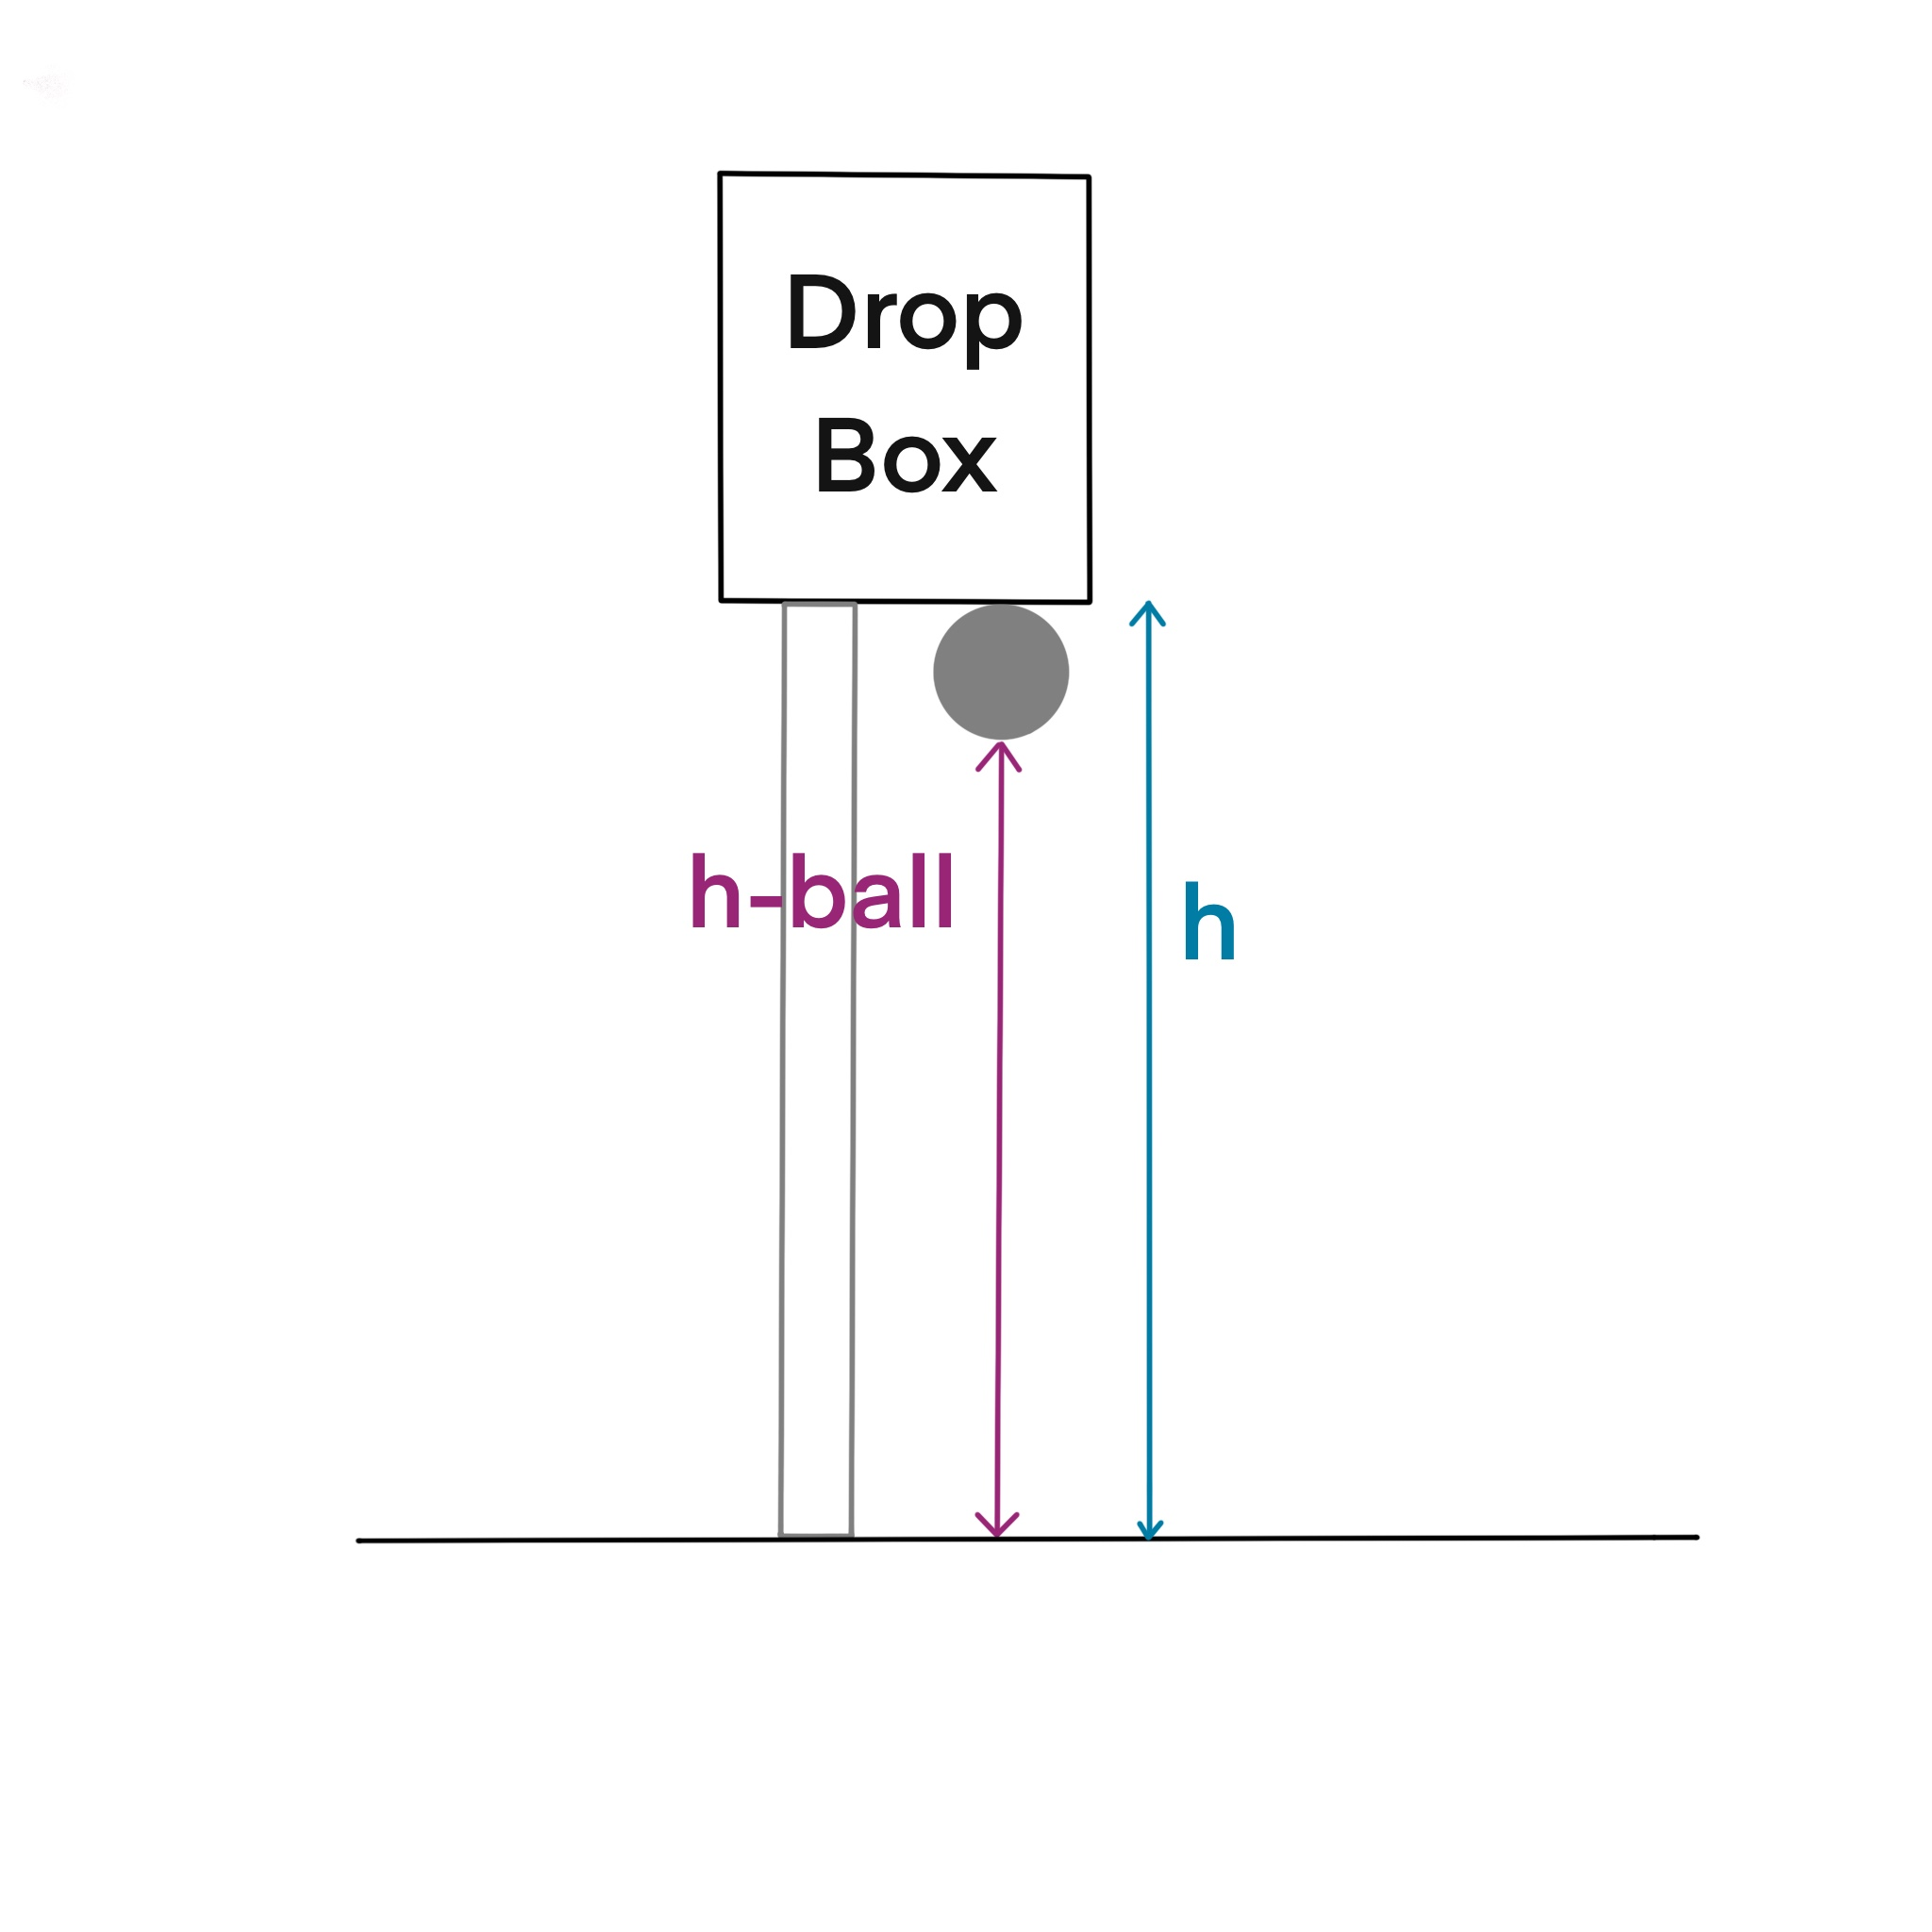
\includegraphics[height=6cm]{./dropbox.jpg}
\captionof{figure}{\label{fig:dropbox}Drop Box setup}
\end{center}

\begin{center}
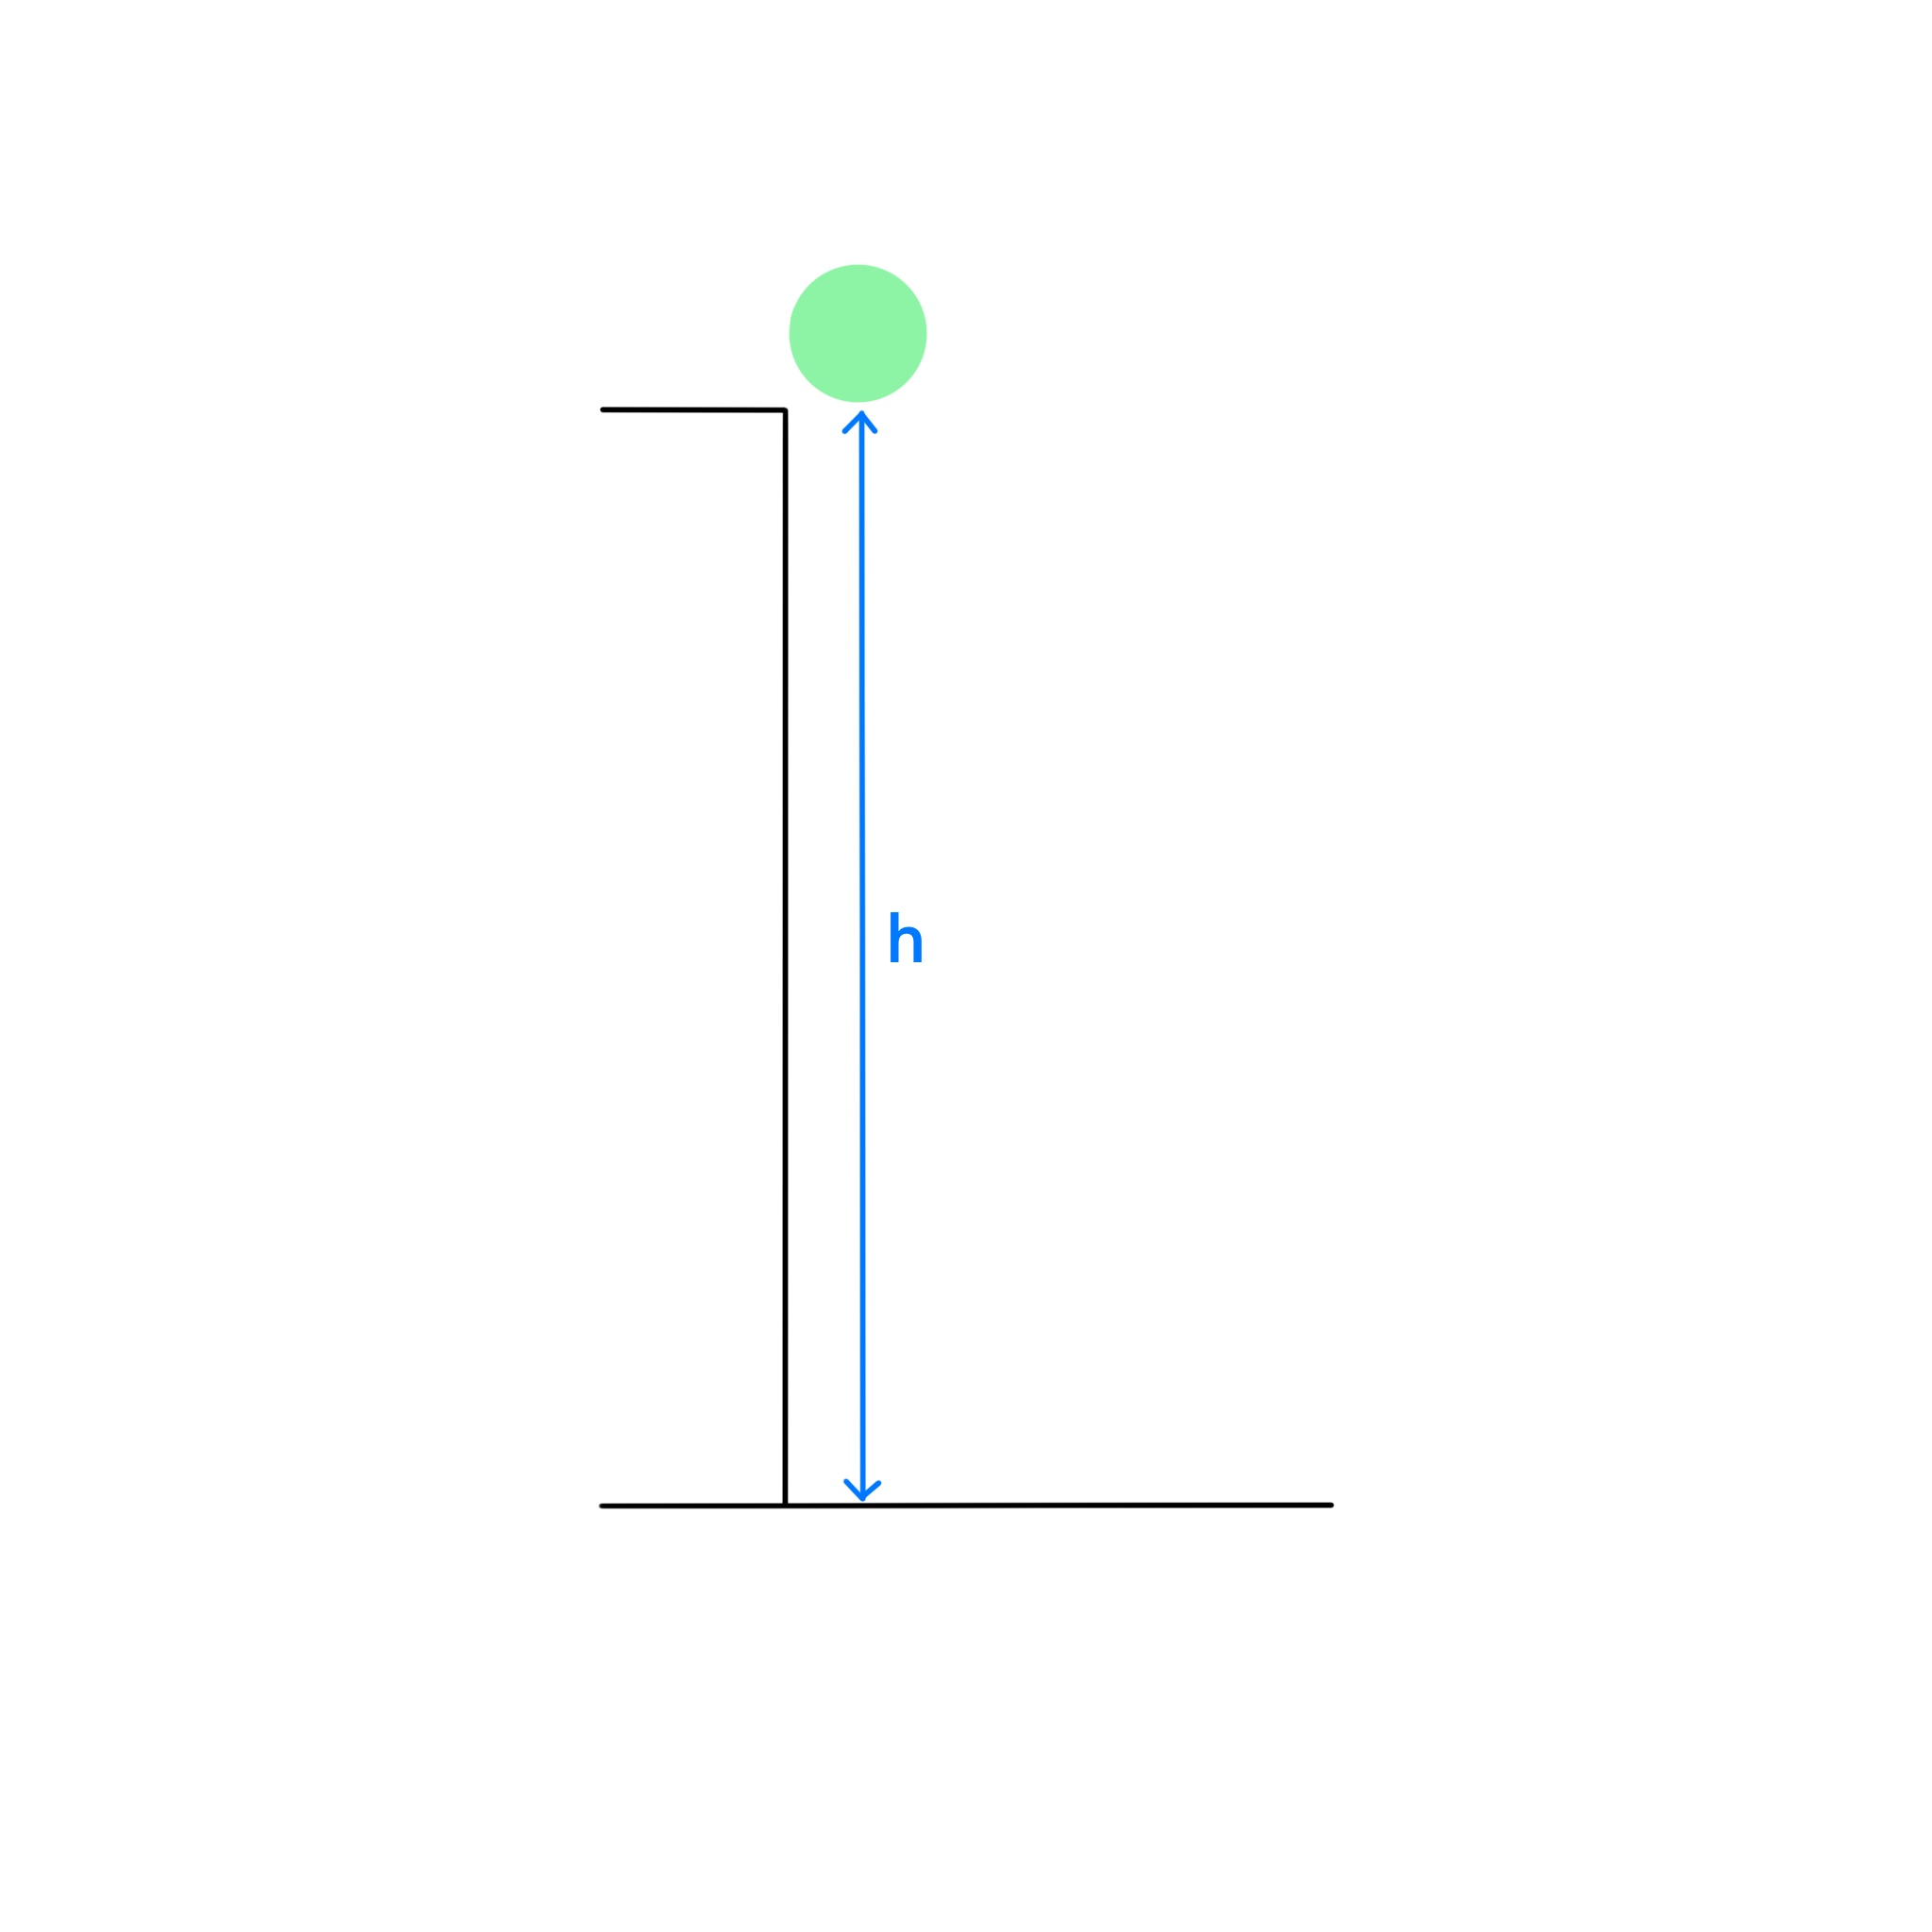
\includegraphics[height=6cm]{./balcony.jpg}
\captionof{figure}{\label{fig:balcony}Balcony drop setup}
\end{center}

Note: the figures are \emph{not} to scale.
\section{Results}
\label{sec:org253cc42}

\subsection{Drop Box}
\label{sec:orgff03c75}

These are the results from the Drop Box experiment.

\begin{center}
\captionof{table}{\label{table:dropbox}Drop Box results}
\begin{tabular}{r|r|r}
Run & Height (cm) & Time (s)\\
\hline
1 & 105.9 & 0.51\\
2 & 105.9 & 0.51\\
3 & 105.9 & 0.51\\
4 & 105.9 & 0.53\\
5 & 105.9 & 0.47\\
\hline
Average & 105.90 & 0.505\\
\end{tabular}
\end{center}

The calculated result of \(g\) using the averages is \(8.3\pm2.3 \frac{\text{m}}{\text{s}^{2}}\).
\subsection{Balcony}
\label{sec:org20ca5a3}

These are the results from the balcony experiment.

\begin{center}
\captionof{table}{\label{table:balcony}Balcony drop results}
\begin{tabular}{r|r|r}
Run & Height (cm) & Time (s)\\
\hline
1 & 560.0 & 1.01\\
2 & 560.0 & 1.05\\
3 & 560.0 & 1.01\\
4 & 560.0 & 1.07\\
5 & 560.0 & 1.00\\
6 & 559.6 & 1.05\\
7 & 560.0 & 1.06\\
8 & 559.6 & 1.06\\
9 & 559.8 & 1.03\\
10 & 560.2 & 1.05\\
\hline
Average & 559.92 & 1.039\\
\end{tabular}
\end{center}

The calculated result of \(g\) using the averages is \(10.4\pm 0.728 \frac{\text{m}}{\text{s}^{2}}\).

All of the calculated results contain the true value of \(g = 9.81 \frac{\text{m}}{\text{s}^{2}}\) within the calculated error propagation.
\section{Discussion}
\label{sec:org0d1f0c8}

Ultimately, the purpose of this lab was to calculate the value of \(g\). The value of \(g\) was obtained in both experiments. However, there is a good amount of error.
\subsection{Calculating error}
\label{sec:org7d98e2e}

Error was calculated using the standard formula for error propagation \(\sigma\): \(\sigma = \sqrt{\sum_{L} \frac{\partial g}{\partial L}^{2}\sigma_{L}^{2}}\) for all measurements \(L\), and \(\sigma_{L}=\sqrt{\sigma_{sys,L}^{2}+\sigma_{res,L}^{2}+\sigma_{stat,L}^{2}}\). Since there are two measurements, height and time, the formula for error propagation is \(\sigma = \sqrt{ \left( \frac{2}{t^{2}} \right) ^{2} \sigma_{h}^{2} + \left( \frac{-4h}{t^{3}} \right)^{2}\sigma_{t}^{2} }\).

The error within a measurement has three components: resolution, systematic, and statistical.

Resolution error is simply half of the resolution of the measuring device. The roll tape has a resolution of 0.2cm, so the resolution error is 0.1cm. For a 30 frames per second video, the resolution is half of the length of a frame, or \(\frac{1}{60}\)s.

Systematic error is the amount of vairability between measurements. For the distance measurements, our group used the resolution error, since we were confident in our measurements of distance. For the video measurements, one frame of error was given for the drop, since noticing the beginning of the ball's movement is tricky, and one frame of error was given for the time it took to hit the ground, since the ball was headed down in one frame and up in the other: the actual bounce was never recorded. This gives two frames of error. For a 30 frames per second video, the systematic error is 2 frames, or \(\frac{2}{30}\)s.

Statistical error is the amount of variability by external factors, such as wind. To account for this vairability, we use the estimate for standard error \(\sigma_{sys} = \frac{\sigma}{\sqrt{n}}\), where \(\sigma\) is the standard deviation of the measurements and \(n\) is the number of measurements.
\subsection{Drop Box error}
\label{sec:org92c71c2}

This result is surprising. Our group expected this to have the smallest total error, but instead it had the largest total error. Here is the calculated error propagation:

\begin{table}[htbp]
\caption{\label{table:dropbox-error}Error propagation for the Drop Box experiment}
\centering
\begin{tabular}{l|r}
\hline
\(\sigma_h\) & 0.0707\\
\(\sigma_{h,sys}\) & 0.05\\
\(sigma_{h,stat}\) & 0\\
\(\sigma_{h,res}\) & 0.05\\
\hline
\(\sigma_t\) & 0.0694\\
\(\sigma_{t,sys}\) & 0.0667\\
\(\sigma_{t,stat}\) & 0.00980\\
\(\sigma_{t,res}\) & 0.0167\\
\hline
\end{tabular}
\end{table}
\end{document}
